\chapter{Auswertung der Ergebnisse und kritische Auseinandersetzung}
\label{ch:Auswertung der Ergebnisse}
Anhand der in dem Teil \ref{ch:Änderungen durch neue Antriebe, Annahmen und Methodik} 
vorgeschlagenen Methodik wurde in diesem Kapitel der Vergleich zwischen 
Referenz-Flugzeugen und alternativen Antrieben geschaffen.
Außerdem werden aufgestellte Betriebsszenarien sowohl ausgewertet, 
schließlich diskutiert und mit anderen Arbeiten verglichenen, 
als auch auf die Vorschläge für andere Arbeiten eingegangen.

\section{Vergleich von Referenzflugzeugen und neuen Antrieben}
\label{s:Ergebnisse_Flugzeuge}
Folgende Erkenntnisse ermöglichen Diskussionen der ersten Hypothese. 
Die Ergebnisse sind nach Flugdistanzen aufgeteilt.\\
%
\subsubsection{Kurzstreckenvergleich: Batterieantrieb und SAF vs. konventioneller Treibstoff}
%
In der Abbildung \ref{vergleichBA_Ref} sind die Ergebnisse der 
batteriebetriebenen ES-19 und der konventionellen L410 dargestellt.
Der Vergleich wurde für 400 Kilometer Flug durchgeführt.
%
Die Gesamtbetriebskosten der ES-19 sind ca. 22 \% höher als die der konventionellen L410, 
wobei der Antrieb mit SAF ein nur 3,6 \% höhere Ergebnis liefert. 
Entgelte und Gebühren bewirken den größten Teil der Betriebskosten aller verglichenen Antriebe, 
gefolgt von kapitalbezogenen Kosten. 
Beim ersten ist ein signifikanter Unterschied zum konventionellen Antrieb zu erkennen, 
und zwar 56 \%, beim zweiten sind das 36 \% höhere Kosten bei Batterieantrieb. 
Der Anteil der Treibstoff- bzw. Energiekosten ist am niedrigsten im Vergleich zu anderen Kosten 
und die Treibstoffkosten sind bei einem konventionellen Flugzeug 30 \% höher. 
Die Treibstoffkosten für SAF sind wesentlich höher (38 \%).

\begin{figure}[h]
	\centering
	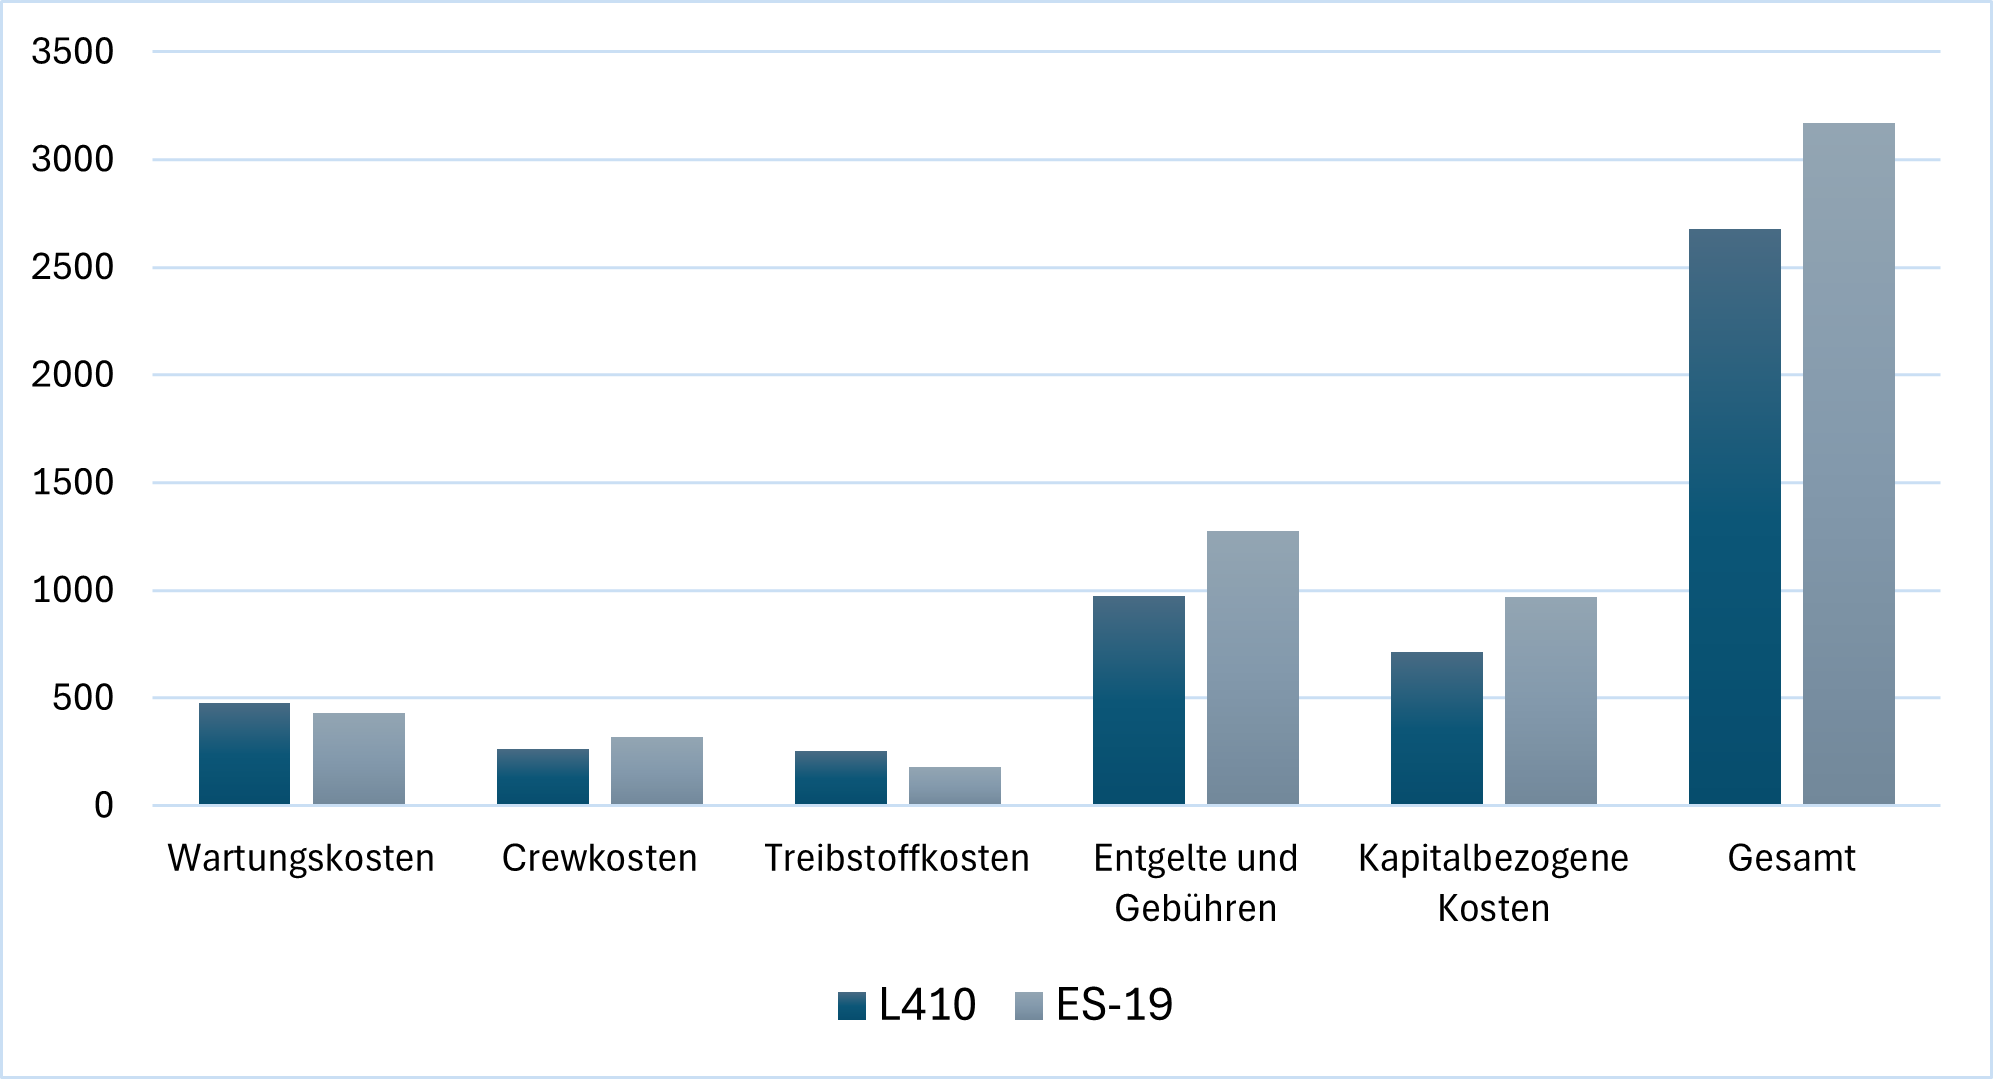
\includegraphics[width=0.9\linewidth]{Bilder/VergleichBA_Ref.png}
	\caption[Betriebskosten]{Vergleich der Referenz und Flugzeug mit der Batterieantrieb und SAF}
	\label{vergleichBA_Ref}
\end{figure}

Zusätzlich zu den Entgelten und Gebühren fallen weitere Abfertigungskosten an,
etwa für den Batteriewechsel oder das Leasing der Batterie für den Flug,
die in die Flughafenentgelte einfließen.
Dieser Wert wird auch in der Sensitivitätsanalyse \ref{s:Sensitivitätsanalyse} überprüft. 
Der Einflusswert für kapitalbezogene Kosten ist der Anschaffungspreis eines Flugzeugs. 
Dieser Wert wurde als weiterer Parameter für die Sensitivitätsanalyse ausgewählt.\\

\subsubsection{Langstreckenvergleich: Wasserstoffantrieb und SAF vs. konventioneller Treibstoff}
In den weiteren Abschnitten wird eine Gegenüberstellung zwischen Flugzeugen mit herkömmlichen Treibstoffen, 
SAF und wasserstoffbetriebener Turbine für einen 6000 Kilometer-Flug durchgeführt. %satz übelstschlecht MAX, nein, war okay :)
Aufgrund der derzeit hohen Wasserstoffpreise wurde zum Vergleich der Wasserstoffmindestpreis 
von 2,1 $EUR/kg$ für das Jahr 2050 herangezogen \cite{hoelzen2022hydrogen}, 
um die mögliche Entwicklung der Wasserstofftechnologien zu beobachten.
%
Das Ergebnis zeigt, dass SAF- und Wasserstoffbetriebene Flugzeuge höhere Betriebskosten haben (siehe \ref{vergleichWA_Ref}).
Die Betriebskosten der Wasserstoffturbine sind rund 40 \% höher, während sie bei SAF um etwa 19 \% höher liegen.
Treibstoff- und kapitalbezogene Kosten haben den größten Einfluss auf die Gesamtkosten, 
Wartungs- und Crewkosten entgegen den geringsten.
Der Einfluss der Entgelte und Gebühren auf die Gesamtkosten ist nicht so groß, 
wie bei den kleineren verglichenen Flugzeugen.
Die Treibstoffkosten für Wasserstoffantrieb sind fast doppelt so hoch (ca. 197 \%), als der für herkömmliche Triebwerke. 
Die Entgelte und Gebühren, Crew- und Wartungskosten haben einen nicht so 
drastischen Unterschied verglichen mit konventionellen Antrieben. 
%
Wird die Entwicklung zukünftiger Preise für Wasserstoff mitbetrachtet, 
kann es sogar zu geringeren Treibstoffkosten im Vergleich zu konventionellen Antrieben führen. 
Die Gesamtbetriebskosten werden weiterhin höher liegen.

%mögliche Hypothese: zukünftige Preisniveau ermöglicht die günstigere Preiswerte
\begin{figure}[h]
	\centering
	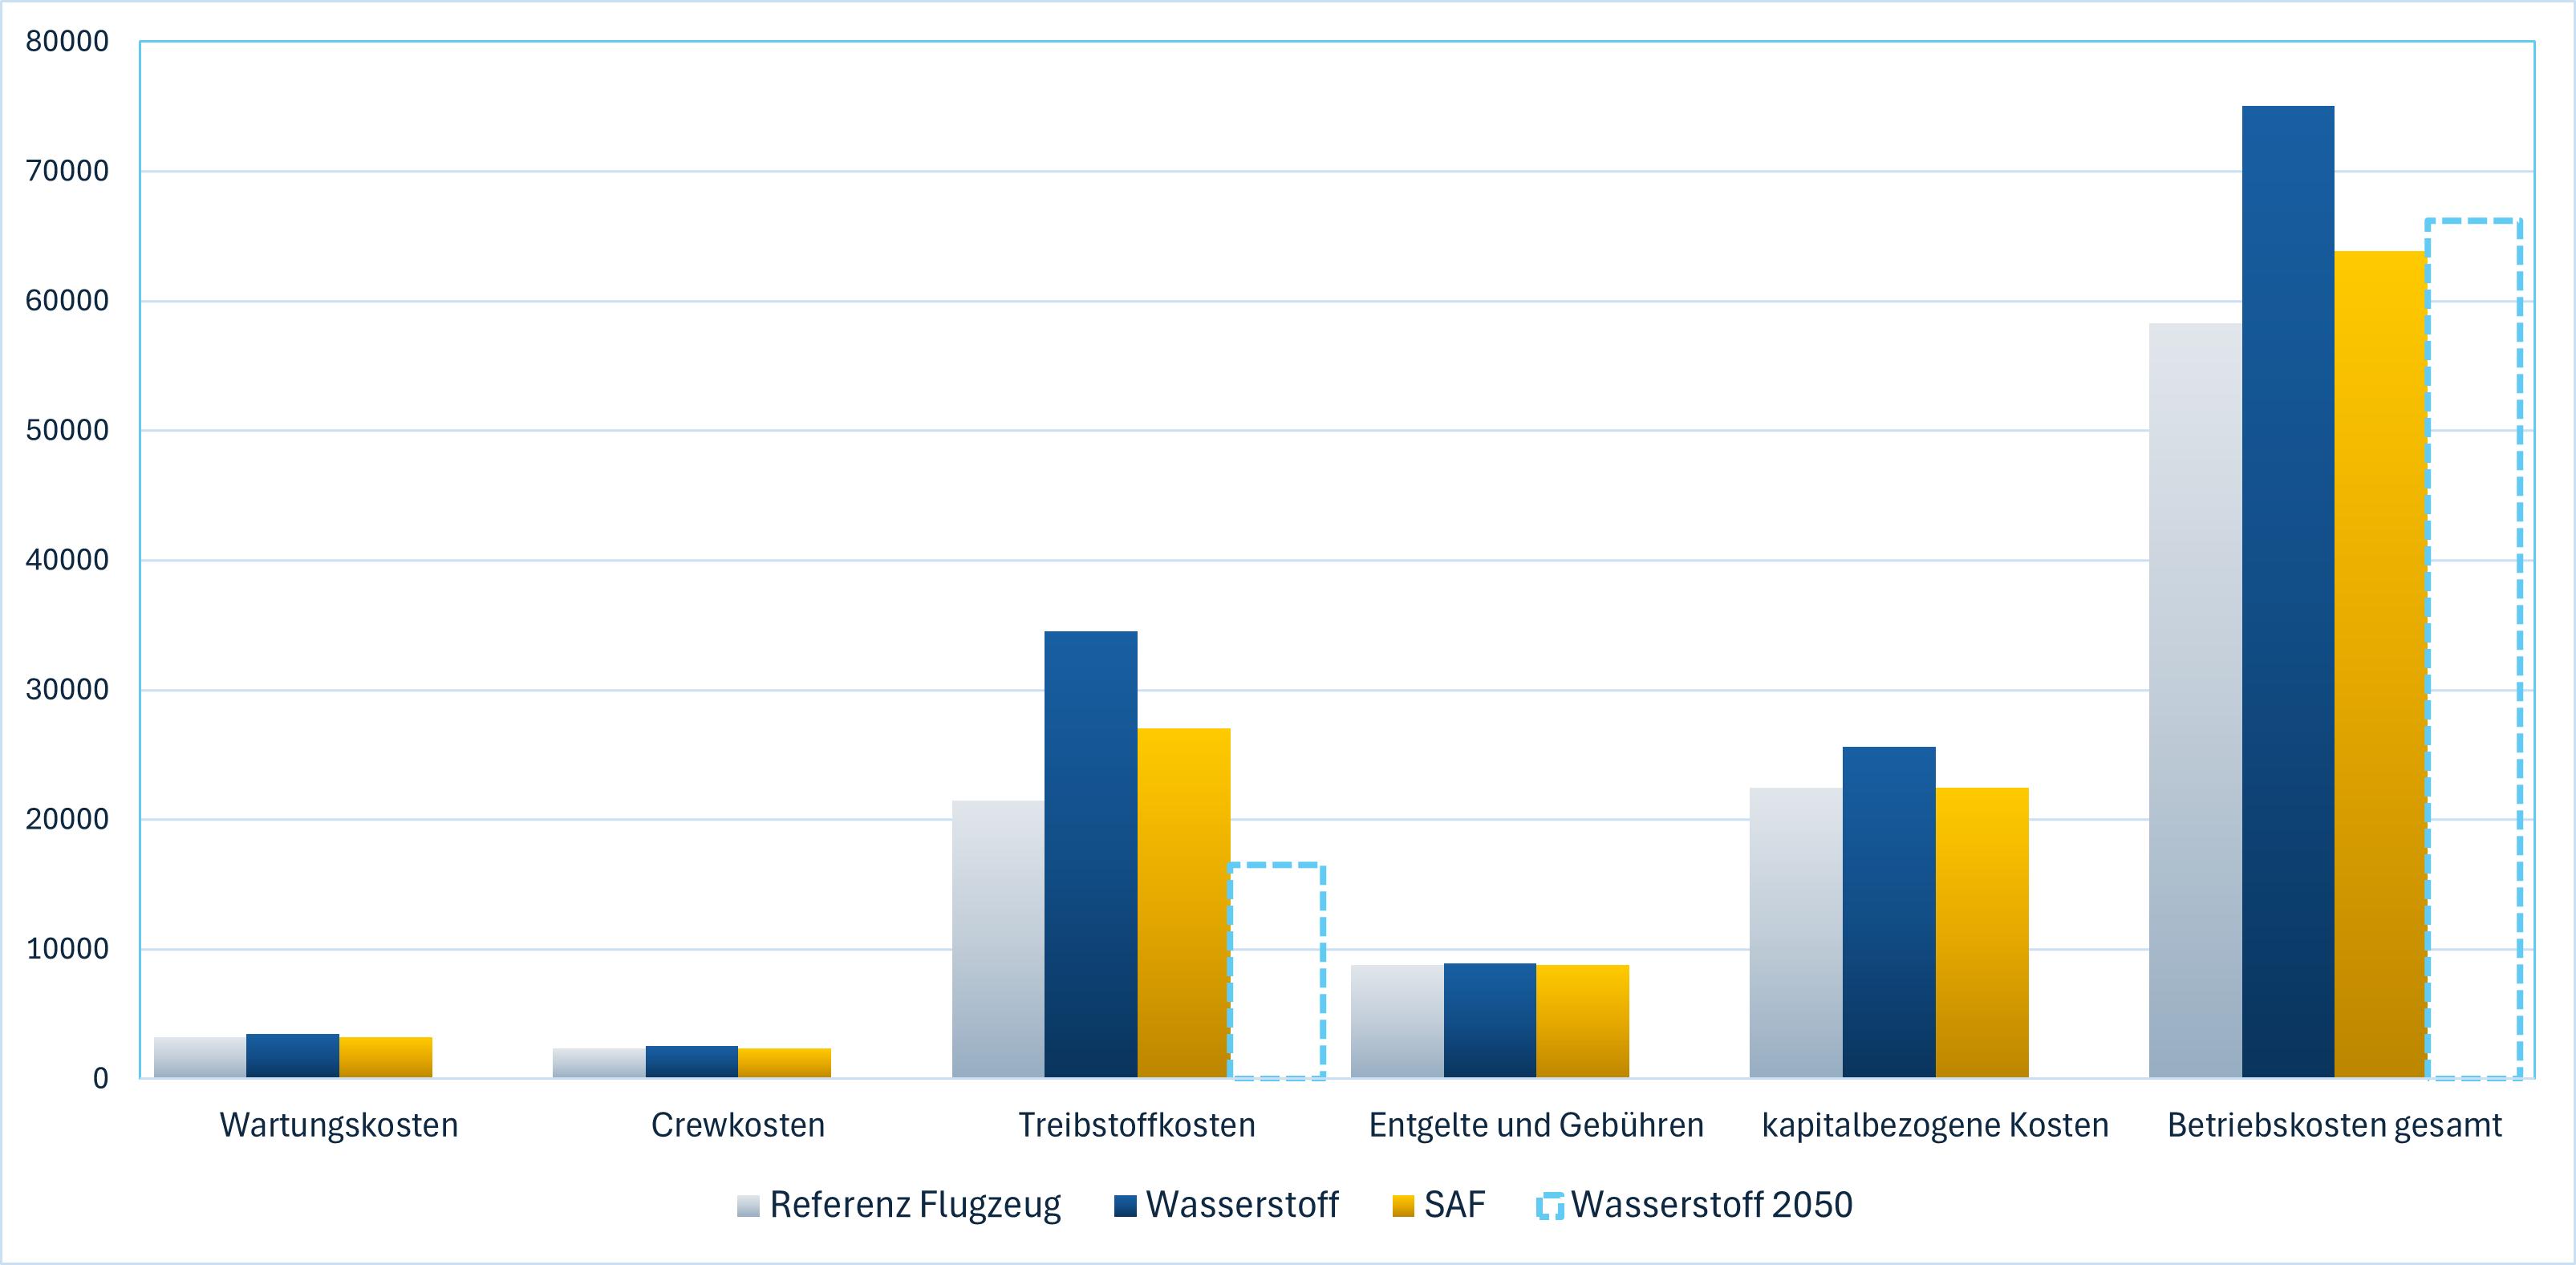
\includegraphics[width=0.9\linewidth]{Bilder/VergleichWA_SAF.png}
	\caption[Betriebskosten]{Vergleich der Referenz und Flugzeug mit der Wasserstoffantrieb und SAF für einen 6000 km Flug}
	\label{vergleichWA_Ref}
\end{figure}

Da die Treibstoffkosten einer der größten Teile in den Ergebnissen ausmachen, 
wird der bedeutsame Parameter Treibstoffpreis für die Sensitivitätsanalyse ausgewählt.
%
Werden Betriebskosten pro Passagierkilometer ausgerechnet und verglichen, 
haben die großen Flugzeuge geringere Kosten als die kleinen Flugzeuge.
Wie auch vorher diskutiert wurde, haben hier konventionelle Treibstoffe 
einen Vorteil sowohl gegenüber den kleinen, als auch großen Flugzeugen.
